\documentclass[10pt]{article}
\usepackage[margin=0.85in]{geometry}
\usepackage{booktabs}
\usepackage{graphicx}
\usepackage{microtype}
\usepackage{amsmath}
\usepackage{enumitem}
\usepackage{hyperref}
\hypersetup{colorlinks=true, linkcolor=blue, citecolor=blue, urlcolor=blue}
\title{Do Visual Grounding Decoders Need Feed-Forward Networks?\\\large A Controlled Study over Frozen Vision-Language Features}
\author{Tarun Tomar\\\small\url{https://github.com/TarunTomar122/attention-is-all-you-need-for-vlms}}
\date{}
\begin{document}
\maketitle

\begin{abstract}
Do feed-forward networks (FFNs) in visual grounding decoders add essential computation once a pretrained vision-language model has already encoded image and language context? We compare a four-block attention-only decoder (A4), a matched four-block attention-plus-FFN decoder (S4), and an eight-block attention-only parameter control (A8) over frozen VLM features. A4 matches or slightly exceeds S4 on RefCOCOg and Ref-Adv-s. FineCops-Ref reveals a small A4 deficit (-0.52 percentage points IoU@0.5, 95\% CI [-0.95, -0.12]), but A8 recovers it (+0.26 points versus S4). Official FineCops levels do not show a monotonic increase in the gap. A4 reduces trainable decoder parameters by 44.4\% and cached-decoder latency by 10.1\%, although end-to-end latency remains backbone-dominated. These results concern the trainable decoder, not a complete attention-only VLM.
\end{abstract}

\section{Introduction}

Visual grounding maps an image and referring expression to one target box. Standard Transformer grounding heads retain attention-plus-FFN blocks, even when their input already contains contextual visual and language features from a pretrained vision-language model (VLM). This leaves a narrow architectural question: once a frozen VLM supplies spatial image features and contextual text states, does a small trainable grounding head still need token-wise FFN computation?

Attention maps can already localize objects, and frozen-LVLM work shows that a few internal heads can be useful for grounding \cite{kang2025heads,wu2025flmm,ding2021vlt}. That does not answer the matched FFN-necessity question. We isolate a new single-query grounding decoder and hold the frozen VLM, data, supervision, readout, box conversion, and evaluation contract fixed.

At fixed depth, A4 removes the FFN residual from each of four decoder blocks and S4 retains it. A8 uses eight attention-only blocks to approximately match S4 trainable parameter count. We ask: (1) does A4 retain S4 performance, (2) does any gap grow with released or official difficulty metadata, and (3) can attention depth recover an observed fixed-depth gap? A4 broadly matches S4 on RefCOCOg and Ref-Adv-s. FineCops-Ref exposes a small gap, but A8 recovers it. The completed slices do not support a monotonic harder-expression boundary.

\section{Why This Comparison Is Non-trivial}

Attention routes a query to relevant text and image tokens, whereas an FFN applies a token-wise nonlinear transformation after routing. If frozen VLM features already encode visual locations and language context, a small head may mostly need retrieval and assembly. But relations, compositional attributes, and distractor resolution could require transformations that attention-only depth cannot reproduce at the same scale.

A global score is insufficient. A4 could match S4 because a dataset is dominated by direct references while losing on relations. An apparent hard-example gap could instead be caused by a changed threshold, a position prior, one-modality shortcut, or performance-defined slice. We use frozen post-processing, paired seeds, modality shuffles, native Ref-Adv metadata, and official FineCops metadata. The RefCOCOg protocol predeclares direct retention and a direct-minus-logical interaction; the latter is not confirmed and is reported as such.

\section{Decoder Intervention}

The frozen SigLIP2 backbone \cite{tschannen2025siglip2} produces 576 image tokens in a $24\times24$ raster grid and contextual text states. Shared learned linear maps project both streams to width 256. A single learned grounding query $q$ alternates text and image cross-attention:
\begin{align*}
q &\leftarrow q + \operatorname{CrossAttentionText}(\operatorname{LN}(q),\operatorname{LN}(T)),\\
q &\leftarrow q + \operatorname{CrossAttentionImage}(\operatorname{LN}(q),\operatorname{LN}(I)).
\end{align*}
S4 then adds $q \leftarrow q + \operatorname{FFN}(\operatorname{LN}(q))$ with a GELU FFN of hidden width 1024. A4 omits this residual and A8 repeats the attention-only block eight times.

The shared readout maps the final query and image tokens to one softmax-normalized patch distribution. Training uses cross-entropy against normalized target-box overlap with each patch. There is no coordinate-regression MLP, segmentation refiner, auxiliary loss, multi-query head, or backbone adaptation.

\begin{figure}[t]
\centering
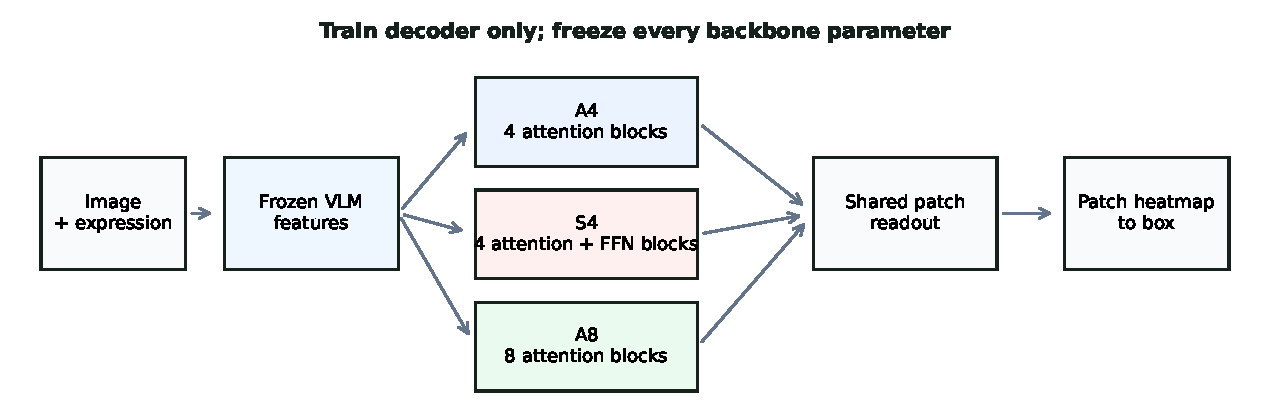
\includegraphics[width=\linewidth]{figures/generated-method-overview.pdf}
\caption{Frozen VLM features feed A4, S4, or A8. The only causal A4/S4 intervention is the decoder FFN residual. The readout and heatmap-to-box conversion are shared.}
\label{fig:method}
\end{figure}

\section{Experimental Protocol}

The heatmap-to-box mass threshold $\tau=0.8$ was selected once on RefCOCOg validation and frozen before every test or out-of-distribution evaluation. Three-seed comparisons average paired seed outputs per example and use 10,000 image-clustered percentile bootstrap replicates with seed 20260812. Image-level resampling retains all expressions associated with a sampled image.

\begin{table}[t]
\centering
\small
\caption{Completed evaluations. RefCOCO and CLIP are descriptive controls.}
\begin{tabular}{p{0.18\linewidth}p{0.21\linewidth}p{0.48\linewidth}}
\toprule
Evaluation & Role & Frozen use \\
\midrule
RefCOCOg UMD & Primary & Three paired seeds, direct/logical protocol, and modality shuffles. \\
RefCOCO UNC & Replication & Seed-0 classic-dataset check. \\
Ref-Adv-s & Adversarial/OOD & 1,142 evaluation-only rows and native metadata slices. \\
FineCops-Ref & Compositional & 9,605 official positive-test rows and official fields. \\
\bottomrule
\end{tabular}
\label{tab:datasets}
\end{table}

The primary metric is box IoU@0.5. Mean IoU, pointing accuracy, and target mass are secondary. Ref-Adv expression-length and distractor-count bins are empirical metadata quartiles defined before performance slicing. FineCops uses released official difficulty and tuple-type fields only. No LLM-derived semantic labels are introduced.

\section{Results}

\begin{table*}[t]
\centering
\caption{Frozen evidence map. Intervals and descriptive labels are preserved rather than collapsed into one significance claim.}
\begin{tabular}{p{0.27\linewidth}rll}
\toprule
Evaluation & A4--S4 (pp) & Interval & Reading \\
\midrule
RefCOCOg direct (3 seeds) & +0.26 & 90\% CI [-0.33, +0.84] & Direct-retention gate passed; interaction not confirmed \\
Ref-Adv-s overall (3 seeds) & +0.79 & 95\% CI [+0.06, +1.52] & No monotonic hard-slice boundary \\
FineCops-Ref overall (3 seeds) & -0.52 & 95\% CI [-0.95, -0.12] & A8-S4 = +0.26 pp \\
CLIP RefCOCOg (1 seed) & +0.18 & descriptive only & Second frozen backbone \\
\bottomrule
\end{tabular}

\label{tab:main}
\end{table*}

\subsection{Standard grounding and modality controls}

On RefCOCOg direct expressions \cite{yu2016context}, A4-S4 is +0.26 pp with a 90\% CI of [-0.33, +0.84]. Direct retention passes, but the planned direct-minus-logical interaction is +1.30 pp with a 95\% CI of [-0.09, +2.66], so it is not confirmed. Correct-pair predictions exceed both image-shuffle and text-shuffle conditions. Correct minus image-shuffle is +48.7 pp for A4 and +48.6 pp for S4; correct minus text-shuffle is +22.6 pp and +22.4 pp. These controls support genuine image/text dependence without establishing a semantic-reasoning boundary.

\subsection{Adversarial grounding}

On Ref-Adv-s \cite{dong2026refadv}, A4-S4 is +0.79 pp (95\% CI [+0.06, +1.52]). Negation, expression length, and distractor count do not show a monotonic A4 loss. The longest-expression quartile is +1.79 pp and the highest-distractor quartile is 0.00 pp. This rejects the expected broad collapse on released metadata, but does not prove equality in every low-count slice.

\subsection{Controlled compositional grounding}

FineCops-Ref \cite{liu2024finecops} supplies the only clear fixed-depth deficit: A4-S4 is -0.52 pp (95\% CI [-0.95, -0.12]). A8-S4 is +0.26 pp. This is compatible with a useful FFN contribution at fixed depth on this benchmark, but not a universal FFN-necessity claim because added attention depth recovers the overall gap. The official level-3 estimate slightly favors A4 but is wide; therefore the official levels do not show a monotonic harder-means-more-FFN-needed trend.

\begin{figure}[t]
\centering
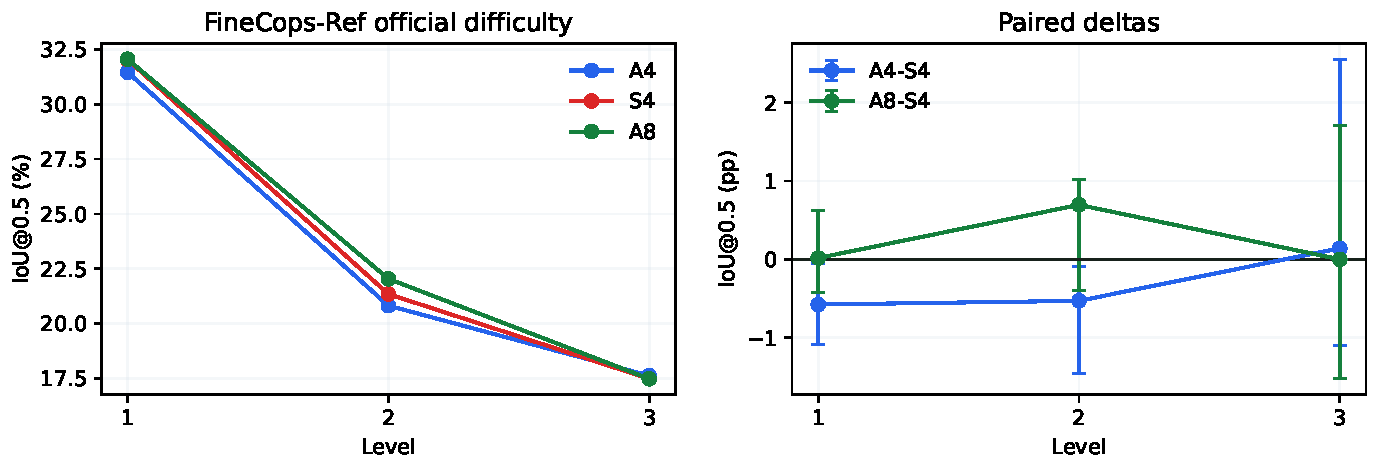
\includegraphics[width=.92\linewidth]{figures/generated-finecops-difficulty.pdf}
\caption{FineCops-Ref official difficulty levels. A4 has a small overall fixed-depth deficit, but level 3 is imprecise and does not support a monotonic hard-example boundary.}
\label{fig:finecops}
\end{figure}

\subsection{Efficiency and second-backbone control}

A4 has 2.64M trainable decoder parameters compared with S4's 4.74M. Cached decoder latency is 6.71 ms versus 7.46 ms, a 10.1\% reduction. Full-pipeline latency is 209.35 ms versus 210.20 ms, so the frozen VLM dominates end-to-end timing. The frozen CLIP one-seed control gives A4-S4 = +0.18 pp; this is directional replication evidence only.

\begin{figure}[t]
\centering
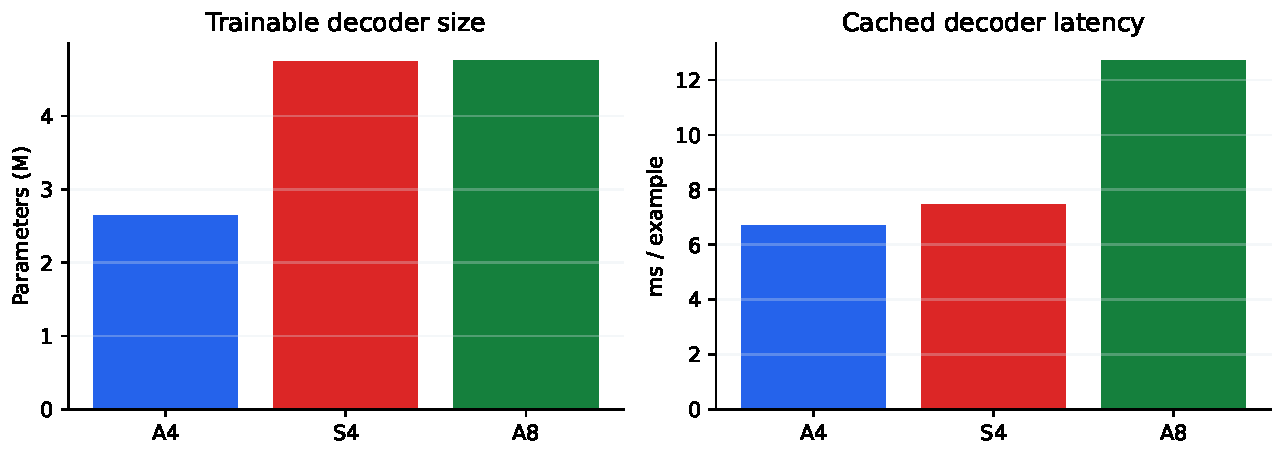
\includegraphics[width=.86\linewidth]{figures/generated-efficiency-summary.pdf}
\caption{A4 reduces trainable decoder size and cached-decoder latency. A8 approximately matches S4 parameters, but is not compute-matched.}
\label{fig:efficiency}
\end{figure}

\section{Related Work and Limits}

Kang et al. \cite{kang2025heads} identify a few localization-relevant heads in a frozen full LVLM. F-LMM \cite{wu2025flmm} uses frozen LMM attention maps but retains CNN and SAM refinement for referring segmentation, while VLT \cite{ding2021vlt} is a referring-segmentation architecture. These precedents establish that attention can expose grounding information but do not perform the matched trainable FFN-deletion ablation over the same frozen image/text tokens. The related attention-only Transformer study in language modeling \cite{ndubuaku2026attention} provides capacity-reallocation context, not direct natural-image grounding evidence.

The frozen backbones retain their FFNs. The output is one box, not pixel segmentation or multi-object detection. The study does not test backbone fine-tuning, multiple learned queries, or complete attention-only VLMs. RefCOCO and CLIP are seed-0/one-seed descriptive replications. A8 recovery shows a viable parameter allocation; it does not identify the mechanism behind every FFN effect.

\section{Conclusion}

FFN deletion is surprisingly benign for a small grounding decoder over frozen VLM features on standard and adversarial referring-expression grounding. A small controlled-compositional deficit appears at fixed depth, but attention depth recovers it and no monotonic difficulty boundary emerges. The supported conclusion is architectural and bounded: attention-only decoder capacity can often substitute for FFN capacity when frozen features already supply relevant visual and language context.

\appendix
\section{Reproducibility Details}

The release is evidence-first. \texttt{scripts/generate\_paper\_assets.py} reads committed bootstrap, slice, efficiency, CLIP-control, and RefCOCOg summary artifacts; it generates manuscript figures, tables, the paper-data manifest, and website images without a GPU or model download. \texttt{scripts/verify\_paper.py} regenerates the artifacts and checks frozen $\tau$, bootstrap configuration, headline values, source hashes, expected assets, and rendered-PDF metadata. \texttt{test\_study.py} checks decoder/data invariants.

The repository releases code, frozen contracts, aggregate result summaries, per-example metric tables where versioned, bootstrap outputs, figures, and decision logs. It excludes third-party images, backbone weights, provider-local checkpoints, and raw qualitative box exports. Qualitative panels must be regenerated from preserved raw predictions and source-attributed images; they must not be inferred from aggregate metrics.

\section{AI Assistance Disclosure}

AI-assisted tools were used for code assistance, experiment orchestration, figure generation, manuscript organization, and language editing. No AI system is an author; responsibility for this manuscript and any eventual submission remains with Tarun Tomar.

\bibliographystyle{plain}
\bibliography{references}
\end{document}
